\chapter{Implementación}
En este séptimo capítulo se presentará la implementación del sistema. En primer lugar, se presentará la estructura del proyecto que se ha realizado en la preparación del frontend y del backend y a continuación
se describirá la implementación de cada una de las funcionalidades del sistema, presentando la documentación de cada ruta de la API y describiendo el código escrito durante el desarrollo.

\section{Estructura del proyecto}
\label{sec:estructura}
Como se mencionó en la arquitectura del sistema en el anterior capítulo, el proyecto se ha desarrollado en dos partes, una parte de frontend y otra de backend. La parte de frontend se ha desarrollado en Flutter y la parte de backend se ha desarrollado en Node.js. 

La estructura del proyecto se puede ver en la siguiente imagen.
\begin{figure}[H]
  \centering
  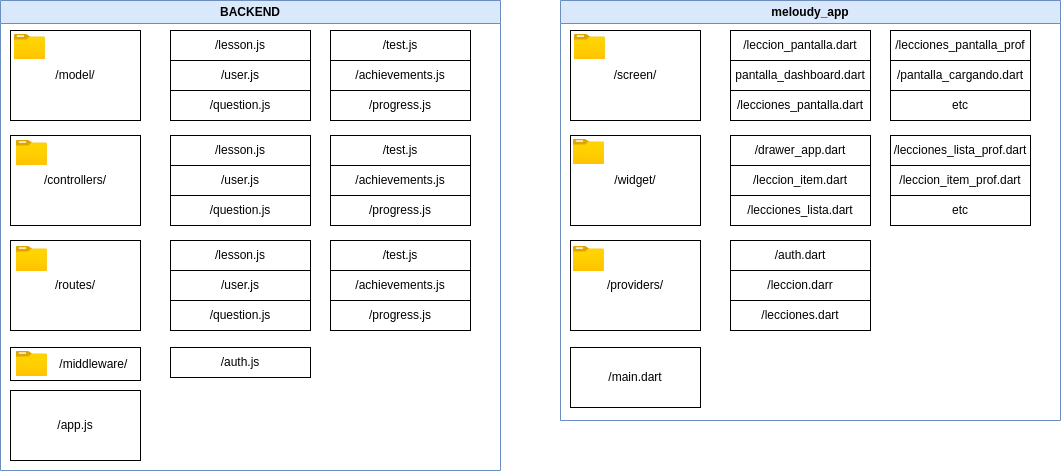
\includegraphics[width=\textwidth]{imagenes/c7/estructura.png}
  \caption{Estructura del proyecto, donde se puede ver la parte de frontend y la parte de backend.}
  \label{fig:login}
\end{figure}

En la figura anterior podemos ver que el desarrollo del proyecto se ha realizado en dos partes, una parte de frontend y otra de backend.

La parte de backend se ha desarrollado en Node.js, por lo que se han dividido los archivos en carpetas de acuerdo a su funcionalidad:
\begin{itemize}
    \item \textit{app.js}: Archivo principal de la aplicación. En él se configura el servidor y se importan las rutas.
    \item \textit{routes}: Carpeta que contiene las rutas de la API. Dentro se encuentran distintos archivos que contienen las rutas de cada entidad de la base de datos (user, lesson, question...).
    \item \textit{controllers}: Carpeta que contiene los controladores de las rutas de la API. Dentro se encuentran distintos archivos que contienen los controladores de cada entidad de la base de datos (user, lesson, question...)
    \item \textit{models}: Carpeta que contiene los modelos de la base de datos.
    \item \textit{middleware}: Carpeta que contiene los middleware de la aplicación. Por dichos middleware pasarán algunas peticiones que se hagan a la API.
\end{itemize}

La parte de frontend se ha desarrollado en Flutter, por lo que se han dividido los archivos en carpetas de acuerdo a su funcionalidad, dentro de la carpeta \textit{lib}:

\begin{itemize}
  \item \textit{main.dart}: Archivo principal de la aplicación. En él se configura la aplicación y se importan las rutas.
  \item \textit{providers}: Carpeta que contiene los providers de la aplicación. Los providers son clases que se encargan de gestionar el estado de la aplicación.
  \item \textit{screen}: Carpeta que contiene las pantallas de la aplicación. Dentro se encuentran distintos archivos que contiene cada pantalla de la aplicación.
  \item \textit{widgets}: Carpeta que contiene los widgets de la aplicación. Dentro se encuentran los archivos de los widgets que se utilizan en las distintas pantallas de la aplicación.
\end{itemize}

\section{Funcionalidad genérica}

\subsection{Drawer}
Se ha implementado un drawer para poder acceder a las pantallas principales de la aplicación y facilitar la navegación por parte del usuario. Este drawer se puede abrir clickando en el icono superior izquierdo de la aplicación. En la siguiente imagen se puede ver el drawer abierto:

\begin{figure}[H]
    \centering
    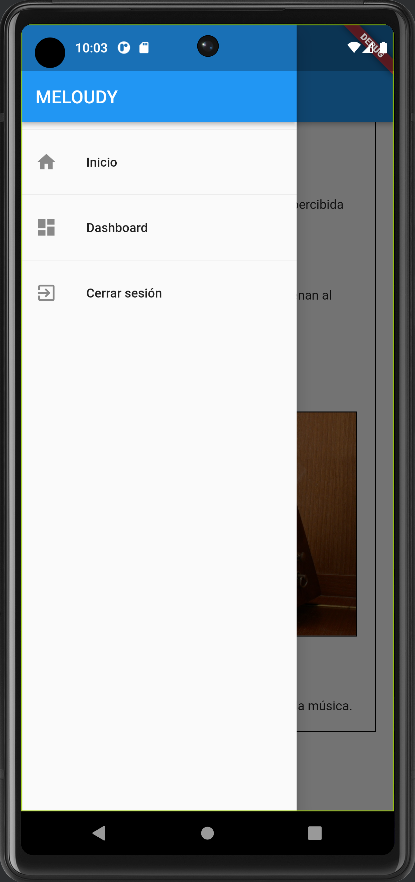
\includegraphics[width=0.4\textwidth]{imagenes/c7/drawer.png}
    \caption{Drawer abierto en la aplicación con tres opciones (por ser desde la vista del profesor): Inicio, Dashboard y Cerrar sesión.}
    \label{fig:login}
\end{figure}


\subsection{Sesión}
\label{sec:sesion}
Se han desarrollado tres características adicionales relacionadas con la sesión de usuario y que explicaremos con más detalle en cada uno de los apartados de la sesión.
\begin{itemize}
    \item Encriptación de la contraseña: La contraseña del usuario se encripta antes de ser almacenada en la base de datos para evitar que sea visible por cualquier persona que tenga acceso a esta. De esta forma
    garantizamos que se cumple el requisito de seguridad de la contraseña.
    \begin{figure}[H]
      \centering
      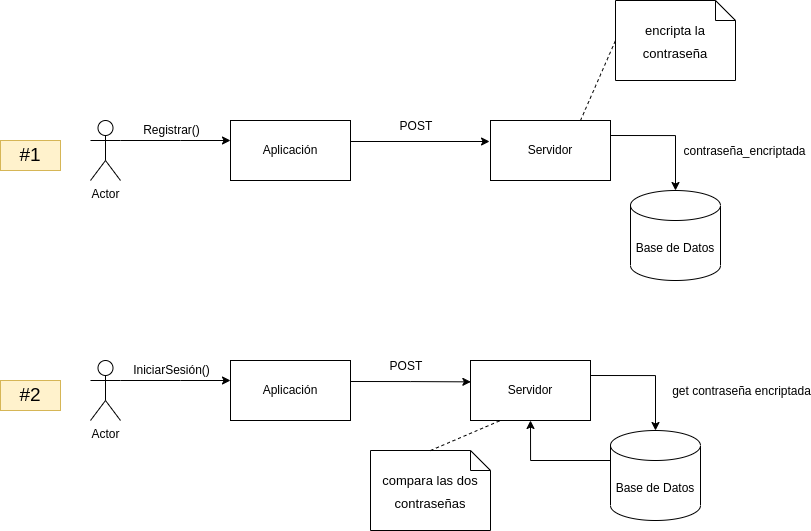
\includegraphics[width=0.8\textwidth]{imagenes/c7/logindiag.png}
      \caption{Diagrama que explica el proceso de encriptación en el inicio de sesión desarrollado en la aplicación.}
      \label{fig:login}
    \end{figure}

    \item Intercambio de token: El servidor proporciona un token al usuario cuando se registra o inicia sesión. Este token se añade a las peticiones que se hagan a la API del. De esta forma, garantizamos que se cumple el requisito de seguridad de la sesión.
    \item Sesión entre instancias: La sesión se mantiene entre instancias de la aplicación. Es decir, si el usuario cierra la aplicación y la vuelve a abrir, no tendrá que volver a iniciar sesión si no ha cerrado la sesión o si el token no ha expirado.
\end{itemize}

\subsubsection{Inicio de sesión}
\textit{Desarrollado en el Sprint 5}

Para el inicio de sesión, el usuario deberá introducir su nombre de usuario y su contraseña. Si el usuario no tiene una cuenta, podrá registrarse pulsando en el botón 'Registrarse'. En la siguiente imagen se puede ver la pantalla de inicio de sesión:
\begin{figure}[H]
    \centering
    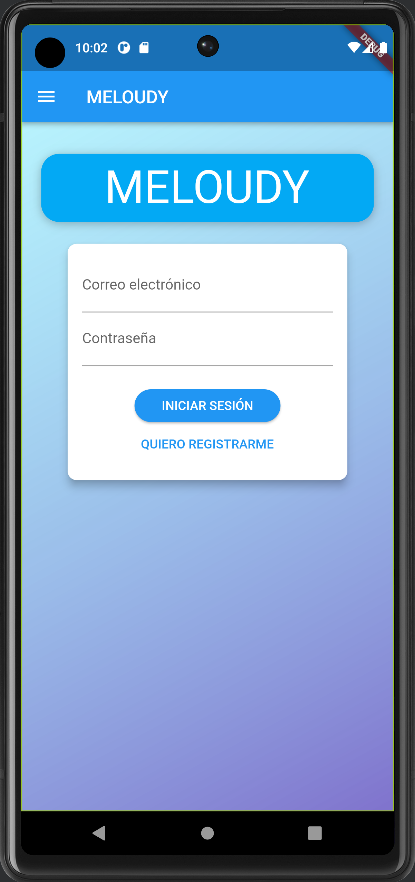
\includegraphics[width=0.4\textwidth]{imagenes/c7/login.png}
    \caption{Pantalla de inicio de sesión}
    \label{fig:login}
\end{figure}

\paragraph*{Vista}
Para la vista, se ha desarrollado un widget para la pantalla de inicio de sesión. Este widget se compone de un formulario con dos campos de texto, uno para el nombre de usuario y otro para la contraseña. Además, el formulario contiene un botón para iniciar sesión y otro para ir a registrarse si el usuario así lo desea.

La pantalla tiene una pila que contiene dos widgets: un container con un fondo en degradado conseguido con el atributo \textit{gradient} de la clase \textit{BoxDecoration} de Flutter, y un SingleChildScrollView que consta de un widget Column para poder colocar los elementos de forma vertical. Dichos elementos son: un container para el título de la aplicación y un widget que contiene el formulario de inicio de sesión (AuthCard()).
AuthCard no es más que un widget Card con dos TextFormField (uno para el correo electrónico y otro para la contraseña) y un ElevatedButton para proceder al inicio de sesión.

\paragraph*{Lógica}
En cuanto a la lógica, una vez el cliente pulsa el botón de 'Iniciar sesión', se llama a la función asíncrona \textit{submit}, la cual se encarga de comprobar que los datos introducidos son correctos.
Cuando los datos son comprobados, se procede a iniciar sesión en la aplicación mediante el método de inicio de sesión del Provider Auth. Para esto, se envia una petición HTTP POST a la ruta \textit{/auth/login} de la API con los datos escritos en el formulario de inicio de sesión.

Por otro lado, en el servidor se ha creado una ruta y una función en el controlador para el inicio de sesión de usuarios. Esta función capta los valores y comprueba que el usuario existe en la base de datos. Si el usuario existe, se comprueba que la contraseña introducida es correcta mediante el método \textit{verify} de bcrypt. Si los datos son correctos, se genera un token de sesión y se devuelve al cliente. Si el usuario no existe o la contraseña es incorrecta, se devuelve un código de estado 400 y un mensaje de error.

\subsubsection{Registro}
\textit{Desarrollado en el Sprint 5}
\paragraph*{Vista}
La vista del registro es muy similar a la del inicio de sesión. La única diferencia es que el formulario contiene un campo adicional para introducir la contraseña de nuevo.
En la siguiente imagen se puede ver la pantalla de registro:
\begin{figure}[H]
  \centering
  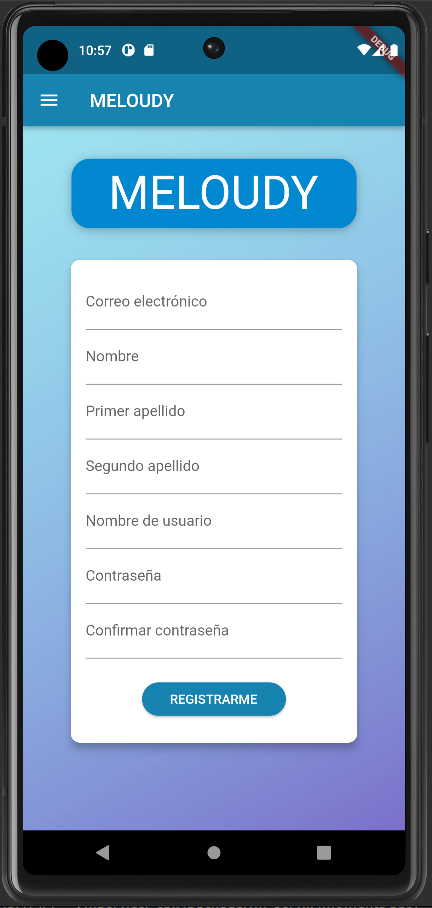
\includegraphics[width=0.35\textwidth]{imagenes/c7/registro.png}
  \caption{Pantalla de registro de los usuarios}
  \label{fig:register}
\end{figure}
\paragraph*{Lógica}
En cuanto a la lógica, una vez el cliente pulsa el botón de 'Registrarse', también se llama a la función asíncrona \textit{submit}, que se encarga de comprobar que los datos introducidos 
son correctos. Cuando se ha hecho esto, si los datos son válidos, la función llama al método de registro del Provider Auth, el cual envia una petición HTTP POST a la ruta \textit{/auth/signup}
 de la API con los datos escritos en el formulario de registro. 

Para poder procesar esta petición de Flutter, se ha creado en el servidor de NodeJS una ruta y una función en el controlador para el registro de usuarios.
 Esta función capta los valores, encripta la contraseña y crea el usuario en la base de datos. Si el registro es correcto,Si los datos son correctos, se genera un token de sesión y
  se devuelve al cliente junto con un código de estado 201 y un mensaje de éxito. Si el registro no es correcto, se devuelve un código de estado 400 y un mensaje de error.

  Cuando Flutter recibe la respuesta del servidor, llama al método \textit{NotifyListeners} del Provider Auth, la cual se encarga de actualizar el estado de la aplicación en las pantallas que estén
  interesadas en los datos de autenticación.

\subsubsection{Cierre de sesión}
\textit{Desarrollado en el Sprint 5}
\paragraph*{Vista}
Para el cierre de sesión, se ha añadido una fila al drawer (barra lateral) de la aplicación, el cual el usuario clickará cuando desee cerrar su sesión.

\paragraph*{Lógica}
La lógica del cierre de sesión es sencilla: se llama a la función \textit{logout} de la clase \textit{Auth} donde se reestablecen los valores de la sesión y se limpian los datos de la sesión almacenados en el dispositivo con el paquete \textit{shared\_preferences}. 
Esta limpieza de datos se realiza en el método \textit{clear}.
Además, se ha añadido un timer que se encarga de cerrar la sesión automáticamente si el token ha expirado. Este timer se ejecuta cada cierto tiempo y comprueba si el token ha expirado. Si es así, se llama al método \textit{logout} mencionado anteriormente.

\section{Funcionalidad de usuario}

\subsection{Lista de lecciones}
\textit{Desarrollado en el Sprint 5}

\label{sec:lista_lecciones}
\paragraph*{Vista}
Para que el usuario pueda ver la lista de lecciones, se ha desarrollado un widget principal para la pantalla. Este widget contiene la ListaLecciones, que a su vez estará compuesta de una lista de widgets llamada LeccionItem. Cada uno de estos widgets contendrá la información principal de una lección, como el título y la imagen de perfil. Además, cada uno de estos widgets (LecciónItem) tendrá un botón para acceder a la lección. En la siguiente imagen se puede ver la pantalla de lista de lecciones: : 

\begin{figure}[H]
  \centering
  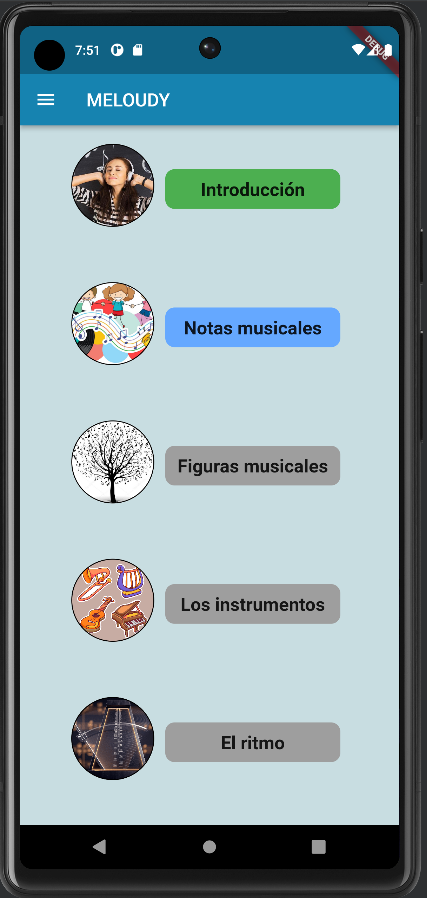
\includegraphics[width=0.4\textwidth]{imagenes/c7/pantprin.png}
  \caption{Pantalla de inicio de sesión}
  \label{fig:login}
\end{figure}

\subsection{Lección} 
\textit{Desarrollado en el Sprint 5}

\label{sec:leccion}
\paragraph*{Vista}
La vista de una lección proporciona al usuario información más detallada de esta. Primero se muestra la imagen de la lección y el título. A continuación, 
se muestra el contenido de la lección en forma de texto, imágenes, vídeos, etc... Esto se ha conseguido construyendo widgets de forma dinámica dependiendo del tipo
de contenido almacenado. Finalmente, se muestra un botón en pantalla para poder hacer un test. En la siguiente imagen se puede ver la pantalla de una lección:

\begin{figure}[H]
  \centering
  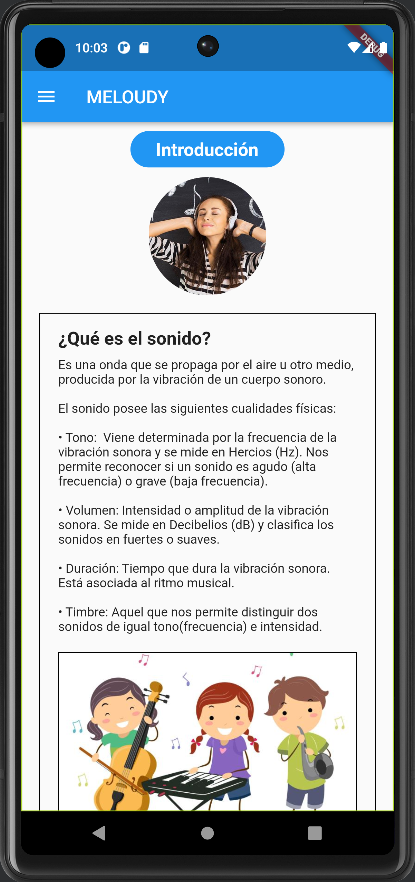
\includegraphics[width=0.4\textwidth]{imagenes/c7/leccion.png}
  \caption{Pantalla de inicio de sesión}
  \label{fig:login}
\end{figure}

  \begin{figure}[H]
    \centering
    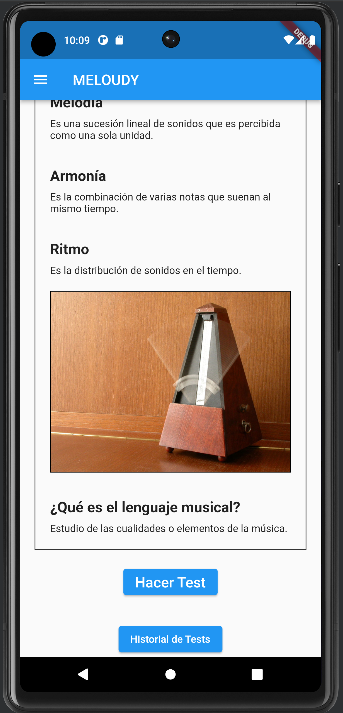
\includegraphics[width=0.4\textwidth]{imagenes/c7/leccion2.png}
    \caption{Pantalla de inicio de sesión}
    \label{fig:login}
\end{figure}

\section{Funcionalidad del profesor}

\subsection{Dashboard}
\textit{Desarrollado en el Sprint 5}

\label{sec:dashboard}
\paragraph*{Vista}
Se ha implementado una pantalla de dashboard para la gestión de la aplicación. En esta pantalla, se muestran las opciones de gestión disponibles para la persona que utiliza la aplicación en función de su rol mediante una columna de ElevatedButton. En la siguiente imagen se puede ver la pantalla de dashboard:

\begin{figure}[H]
  \centering
  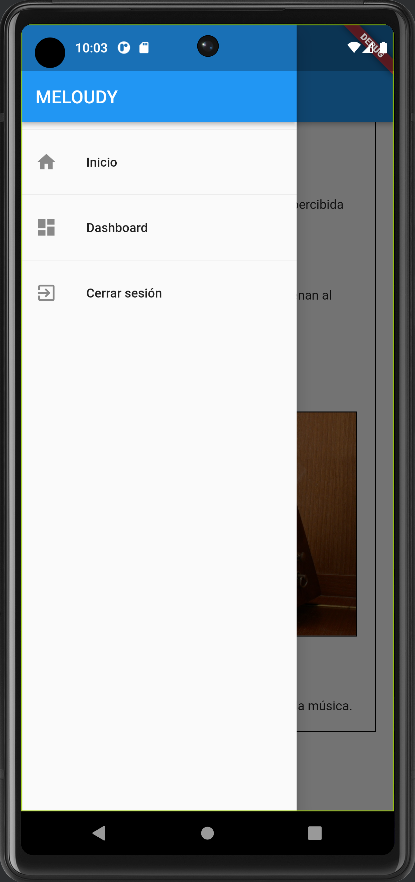
\includegraphics[width=0.4\textwidth]{imagenes/c7/drawer.png}
  \caption{Pantalla de inicio de sesión}
  \label{fig:login}
\end{figure}


\subsection{Lista de lecciones} 
\textit{Desarrollado en el Sprint 5}

\paragraph*{Vista}
La lista de lecciones del profesor es muy similar a la del usuario. Las diferencias, aparte de los estilos, son los botones de tipo ElevatedButton que se han añadido para la gestión de las lecciones y que permiten al profesor crear y eliminar lecciones. En la siguiente imagen se puede ver la pantalla de lista de lecciones del profesor:

\begin{figure}[H]
  \centering
  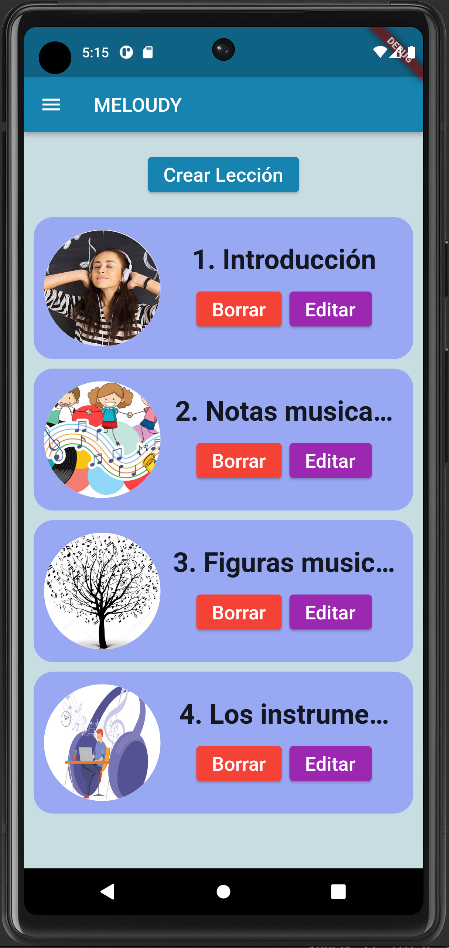
\includegraphics[width=0.4\textwidth]{imagenes/c7/listalecciones.png}
  \caption{Pantalla de inicio de sesión}
  \label{fig:login}
\end{figure}